\documentclass[10pt]{../usamts}

\realname{Juni Kim}
\username{junikimm}
\usamtsid{38002}
\usamtsyear{35}
\usamtsround{3}

\begin{document}

%%%%%%%%%%%%%%%%%%%%%%%%%%%%%%%%%%%%%
%%%%%%%%%%                 %%%%%%%%%%
%%%%%%%%%%    Problem 1    %%%%%%%%%%
%%%%%%%%%%                 %%%%%%%%%%
%%%%%%%%%%%%%%%%%%%%%%%%%%%%%%%%%%%%%
\begin{solution}

\begin{center}
\begin{asy}
size(10cm);
bool DRAW_SOLUTION = true;

int n = 6;
real LINE_WIDTH = 0.3;
void drawHLine(int x, int y) {
fill((x,y+0.5-LINE_WIDTH/2)--(x,y+0.5+LINE_WIDTH/2)--(x+1,y+0.5+LINE_WIDTH/2)--(x+1,y+0.5-LINE_WIDTH/2)--cycle, gray(0.8));
}
void drawVLine(int x, int y) {
fill((x+0.5-LINE_WIDTH/2,y)--(x+0.5+LINE_WIDTH/2,y)--(x+0.5+LINE_WIDTH/2,y+1)--(x+0.5-LINE_WIDTH/2,y+1)--cycle, gray(0.8));
}
void drawNum(int x, int y, int num) {
label(scale(2.5)*string(num), (x+0.5,y+0.5));
}
void drawSolNum(int x, int y, int num) {
if (DRAW_SOLUTION) {
drawNum(x, y, num);
}
}
drawHLine(2,0);
drawHLine(4,1);
drawHLine(1,2);
drawHLine(3,2);
drawHLine(4,3);
drawHLine(2,4);
drawHLine(3,5);
drawVLine(0,4);
drawVLine(1,3);
drawVLine(2,1);
drawVLine(2,3);
drawVLine(3,4);
drawVLine(4,1);
drawVLine(5,2);

drawNum(0, 0, 5);
drawNum(4, 0, 3);
drawNum(1, 2, 2);
drawNum(3, 3, 4);
int[][] numbers =
{{6,1,3,5,4,2},
{2,6,5,3,1,4},
{3,5,1,4,2,6},
{4,2,6,1,5,3},
{1,3,4,2,6,5},
{5,4,2,6,3,1}};

for(int i = 0; i <= 6; i += 1) {
draw((i,0)--(i,6));
draw((0,i)--(6,i));
}

for(int i=0;i<6; i += 1){
for(int j=0;j<6;j += 1){
if(!(i == 3 & j == 3 | i == 0 & j == 0 | i == 4 & j == 0 | i == 1 & j == 2)){
drawSolNum(i,j,numbers[5-j][i]);
}
}
}
\end{asy}
\end{center}
\end{solution}

%%%%%%%%%%%%%%%%%%%%%%%%%%%%%%%%%%%%%
%%%%%%%%%%                 %%%%%%%%%%
%%%%%%%%%%    Problem 2    %%%%%%%%%%
%%%%%%%%%%                 %%%%%%%%%%
%%%%%%%%%%%%%%%%%%%%%%%%%%%%%%%%%%%%%

\begin{solution}

Without loss of generality, let $a=1$. Then there are no interior points, so the problem condition cannot hold. Thus, we can assume $a,b,c \geq 2$.

The number of unpainted cells is $(a-2)(b-2)(c-2)$. There are clearly $2 \cdot \paren{(a-2)(b-2)+(b-2)(c-2)+(a-2)(c-2)}$ cells that are painted exactly once, $4 \cdot \paren{(a-2)+(b-2)+(c-2)}$ cells that are painted exactly twice, and $8$ corners which are each painted thrice.

The problem asks us to find all $a,b,c$ such that $5(a-2)(b-2)(c-2) = abc$. Without loss of generality, let $a \le b \le c$.
Rearranging some of the terms, we get that $\frac{5(a-2)}{a} = \frac{b}{b-2} \cdot \frac{c}{c-2} \le \frac{b^2}{(b-2)^2}$.

We now observe that $a$ is upper bounded by 4. Consider if this were not the case; $3 \le \frac{5(a-2)}{a}$ and $\frac{b^2}{(b-2)^2} \le \frac{25}{9} < 3$. So, the above inequality cannot hold, which is a contradiction.

Consider the case where $a=3$. Then $b \leq 8$. Consider if this were not the case; $\frac{5(a-2)}{a} = \frac{5}{3}$ but $\frac{b^2}{(b-2)^2} \leq \frac{9^2}{7^2} < \frac{5}{3}$, which contradicts our original inequality condition.

Consider the case where $a=4$. Then $b \leq 5$. Consider if this were not the case; $\frac{5(a-2)}{a} = \frac{5}{2}$ but $\frac{b^2}{(b-2)^2} \leq \frac{6^2}{4^2} < \frac{5}{2}$, which contradicts our original inequality condition.

Now, we are left with a finite case check:

\begin{center}
\begin{tabular}{c | c | c}
    $(a,b)$ & Required value of $1-\frac{2}{c}$ & Value of $c$\\\hline
    $(3,3)$ & 9/5 & $-\frac{5}{2}$ \\
    $(3,4)$ & 6/5 & $-10$ \\
    $(3,5)$ & 1 & undefined \\
    $(3,6)$ & 9/10 & $20$ (valid) \\
    $(3,7)$ & 21/25 & $\frac{25}{2}$ \\
    $(3,8)$ & 4/5 & $10$ (valid) \\
    $(4,4)$ & 4/5 & $10$ (valid) \\
    $(4,5)$ & 2/3 & $6$ (valid) \\
\end{tabular}
\end{center}

Upon inspection, it is clear that the only possible solutions are the integer triples $(3,6,20)$, $(3,8,10)$, $(4,4,10)$, $(4,5,6)$ and their permutations, which all work.

\end{solution}


%%%%%%%%%%%%%%%%%%%%%%%%%%%%%%%%%%%%%
%%%%%%%%%%                 %%%%%%%%%%
%%%%%%%%%%    Problem 3    %%%%%%%%%%
%%%%%%%%%%                 %%%%%%%%%%
%%%%%%%%%%%%%%%%%%%%%%%%%%%%%%%%%%%%%
\begin{solution}
We claim that the answer is all $n$ such that \fbox{$3 \nmid n$}.

Let $(a,b)$ denote a game state where we have $a$ ones and $b$ twos. The number of zeroes is irrelevant since they are already out of consideration from our game.
Call a game state \textit{maintainable} if either:
\begin{enumerate}
    \item $a = 1$ and $b \equiv 1 \pmod 3$
    \item $a = 0$ and $b \equiv 0 \pmod 3$
\end{enumerate}

Note that the ultimate losing game state, $(0,0)$ is maintainable. Now, the pith of our solution is the following lemma:
\begin{claim}
    Without loss of generality, let it be Lizzy's turn. If the game state is \textit{maintainable}, Alex, no matter what legal move Lizzy plays, can always make the game state \textit{maintainable} after his turn.
\end{claim}
\begin{proof}
    First, we case bash on Lizzy's moves when the game state is denoted as $(1, 3m+1)$ for some non-negative integer $m$.
    If she decides to delete a two (that is, turn it into a zero), the game state becomes $(1, 3m)$. In this case, Alex can clearly just delete a one to turn the game state into $(0,3m)$.

    Now, there are three different cases where Lizzy chooses to decrement some number of twos, but decides to keep the one that was already there.
    \begin{itemize}
        \item She decrements $3n$ twos; the game state is then $(3n+1, 3(m-n)+1)$. Alex can then delete $3n$ of the ones (this is possible since $n$ in this particular case is forced to be nonzero) and turn the game state into $(1, 3(m-n)+1)$.
        \item She decrements $3n+1$ twos; the game state is then $\paren{3n+2, 3(m-n)}$. Alex can then decrement all the ones on the board to make the game state $(0,3(m-n))$.
        \item She decrements $3n+2$ twos; the game state is then $\paren{3n+3, 3(m-n)-1}$. Alex can then decrement all of the ones on the board and decrement a two, altering the game step as follows: $(3n+3, 3(m-n)-1) \Rightarrow (0,3(m-n)-1) \Rightarrow (1, 3(m-n)-2)$.
    \end{itemize}
    There are also three different cases (basically the same logic) where she deletes the one that was already on the board and decrements some number of twos.
    \begin{itemize}
        \item She decrements $3n$ twos; the game state is then $(3n, 3(m-n)+1)$. Alex can then delete $3n-1$ of the ones and turn the game state into $(1, 3(m-n)+1)$. In the case that $n=0$, Alex can delete a two to turn the game state into $(0, 3(m-n))$.
        \item She decrements $3n+1$ twos; the game state is then $\paren{3n+1, 3(m-n)}$. Alex can then decrement all the ones on the board to make the game state $(0,3(m-n))$.
        \item She decrements $3n+2$ twos; the game state is then $\paren{3n+2, 3(m-n)-1}$. Alex can then decrement all of the ones on the board and decrement one of the twos, altering the game step as follows: $(3n+3, 3(m-n)-1) \Rightarrow (0,3(m-n)-1) \Rightarrow (1, 3(m-n)-2)$.
    \end{itemize}

    Next, we case bash on Lizzy's moves when the game state is denoted as $(0, 3m)$ for some positive integer $m$.
    If she decides to delete a two, the game state becomes $(0, 3m-1)$. Alex can just decrement a two to turn the game state into $(1, 3m-2)$.

    Now, there are three different cases where Lizzy decrements a certain number of twos from the board (this number must be positive):
    \begin{itemize}
        \item She decrements $3n$ twos; the game state is then $(3n, 3(m-n))$. Alex can decrement all the ones and turn the game state into $(0, 3(m-n))$.
        \item She decrements $3n+1$ twos; the game state is then $(3n+1, 3(m-n)-1)$. Alex can decrement all of the ones and decrement a two, turning the game state into $(1, 3(m-n)-2)$.
        \item She decrements $3n+2$ twos; the game state is then $(3n+2, 3(m-n)-2)$. Alex can decrement all but a single one, turning the game state into $(1, 3(m-n)-2)$.
    \end{itemize}
\end{proof}

Note that both the number of twos and the sum of all the numbers in the game are strictly decreasing monovariants. From the case bash we just did, it is also apparent that the other player will never be on a \textit{maintainable} state. Therefore, the sum of all numbers in the game will eventually go to zero, and it will then be the turn of the player on the \textit{maintainable} state, at which point they lose. If the state it \textit{maintainable} on a player's turn, they are on a death spiral.

Now, if $n$ is a multiple of 3, Lizzy is already on this death spiral, and therefore she will lose. If $n$ is not, Lizzy can make one of the following two moves to force Alex onto the death spiral:

\begin{itemize}
    \item If $n = 3k+1$; Lizzy can delete a two, turning the game state from $(0, 3k+1)$ to $(0, 3k)$.
    \item If $n = 3k+2$; Lizzy can decrement a two, turning the game state from $(0,3k+2)$ to $(1,3k+1)$.
\end{itemize}

\end{solution}

%%%%%%%%%%%%%%%%%%%%%%%%%%%%%%%%%%%%%
%%%%%%%%%%                 %%%%%%%%%%
%%%%%%%%%%    Problem 4    %%%%%%%%%%
%%%%%%%%%%                 %%%%%%%%%%
%%%%%%%%%%%%%%%%%%%%%%%%%%%%%%%%%%%%%
\begin{solution}

We first solve \textbf{Part a}, for which the statement is \fbox{true}. It is well-known that the cardinality of $\RR^n$ is the same as the cardinality of any open interval $(a,b)$ on the real line. Therefore, there exists some bijection which maps $\RR^2$ to $(0,2\pi)$. We can then map elements on $(0,2\pi)$ to a unique point on the unit circle of the complex plane: $x \hookrightarrow e^{xi}$. Any polygon with vertices on this unit circle, if it is not self-intersecting, is immediately convex. Therefore, any polygon on our original plane will get mapped to a convex polygon which is not degenerate (because of injectivity).


We now solve \textbf{Part b}, for which the statement is \fbox{false}. We will consider a regular 1001-gon with all points on the unit circle. Any polygon that is generated with a subset of the vertices of this 1001-gon, assuming no self-intersections, is also convex.
\begin{claim}
    Let $G^*$ be the image of a convex polygon $G$ under the map $f$ whose points are all on the unit circle. Then, $G^*$ cannot have any convex sub-polygon with more than 3 points. In particular, its convex hull, if it has more than three points, must be a triangle.
\end{claim}
\begin{proof}
    If there exists a convex sub-polygon on $G^*$ which contains more than 3 points, let it be temporarily denoted $S^*$, we can just take the intersection of $G$ and the pre-image of $S^*$ to get a set of points that denote a convex polygon but whose image is also a convex polygon. The convex hull must be a triangle because otherwise we get a degenerate quadrilateral on a line, which is not allowed
\end{proof}

\begin{claim}
    The image of the vertices of a regular 1001-gon under the map $f$ must contain at least 250 distinct points.
\end{claim}
\begin{proof}
    Assume for the sake of contradiction that this was not true. Then, there exists a point $x$ such that at least 5 vertices of our 1001-gon map to it. Now, consider the set of all vertices $v$ such that $f(v) = x$, which we denote as $V$. The points in $V$ form a convex polygon with at least 5 sides, but the image of $V$ is a single point, which is a degenerate polygon.
\end{proof}

Therefore, we can find points $A$, $B$, $C$, $D$, $E$, and $F$ such that they all map to different points under $f$. Without loss of generality, let $A^*$, $B^*$, and $C^*$ be the points on the convex hull of the image of $ABCDEF$ (By our previous claim, these are the only points on the convex hull). Then, $D^*$, $E^*$, and $F^*$ must be points inside this convex hull. Consider the following diagram:

\begin{center}
    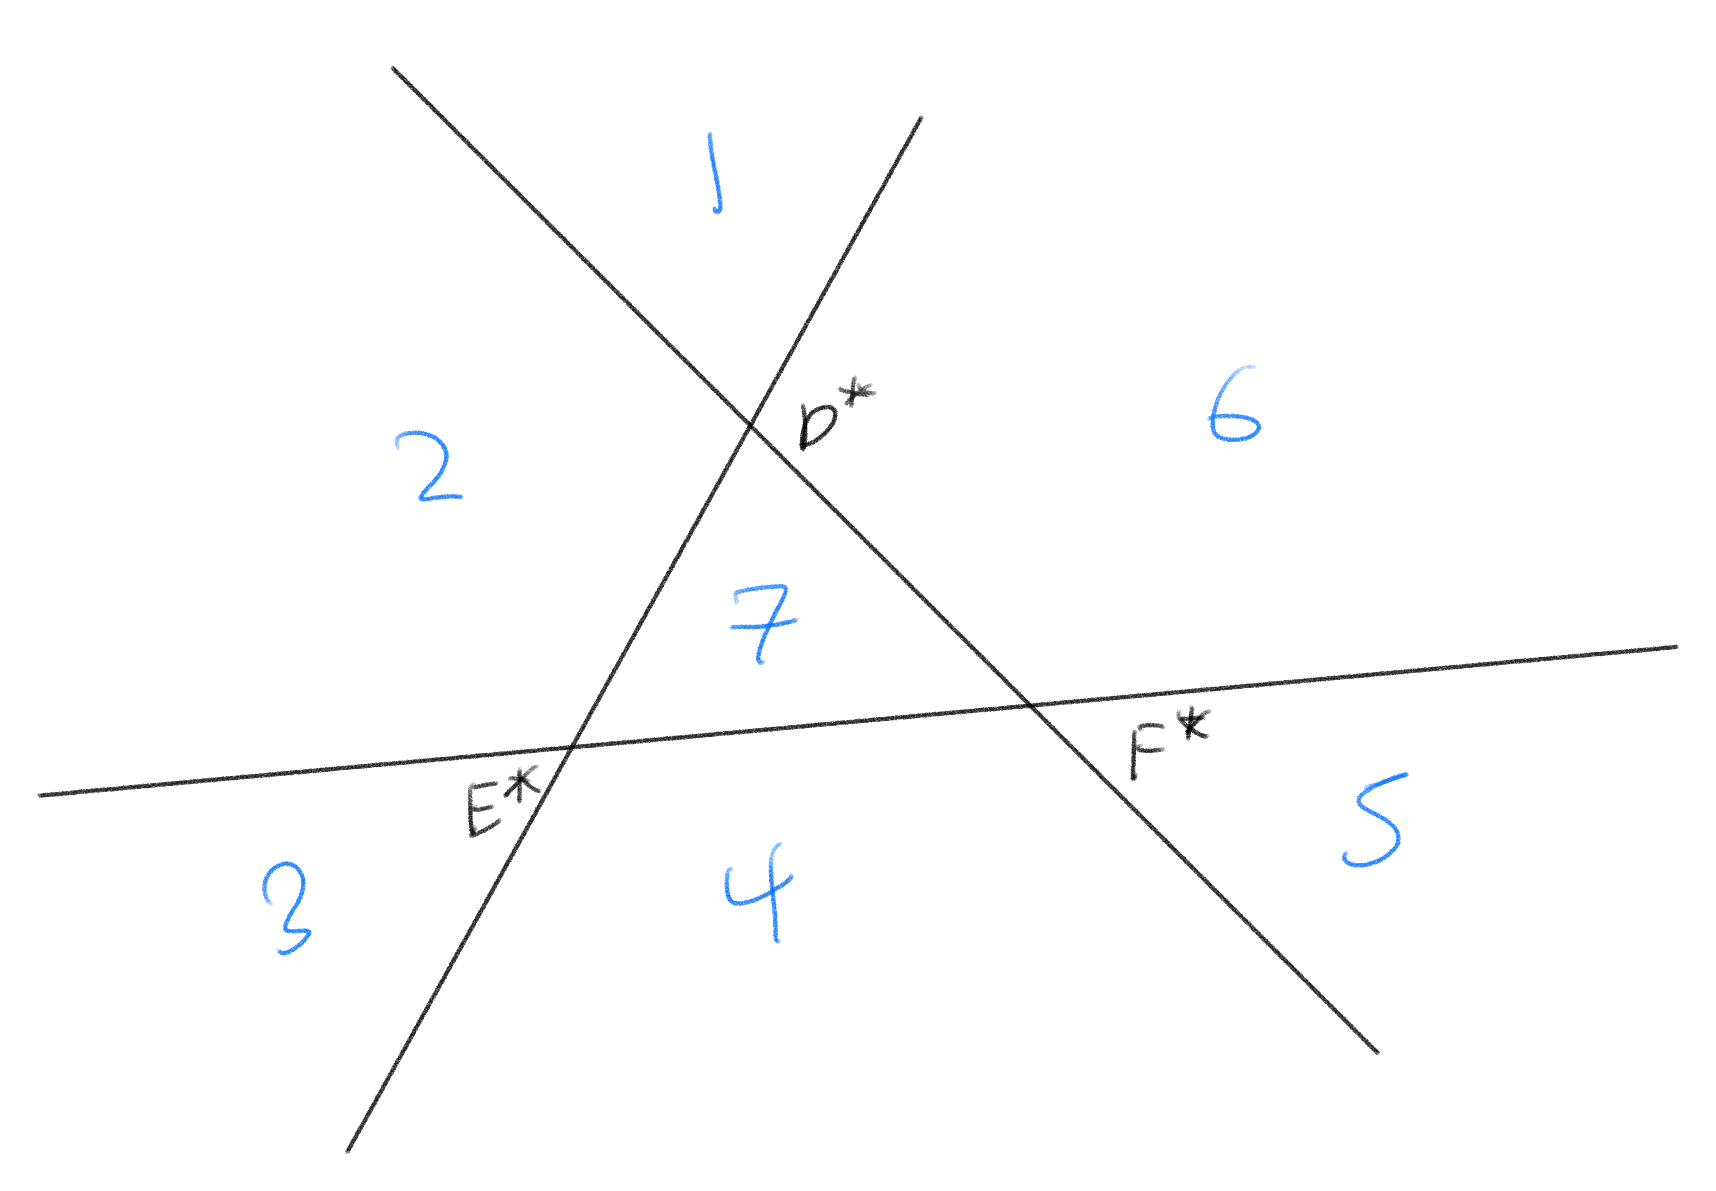
\includegraphics[width=8cm]{round3/p4diagram.jpeg}
\end{center}

Because $A^*$ is part of the convex hull, it cannot be inside region 7, in which case it would fail to be part of the convex hull. The same reasoning applies for $B^*$ and $C^*$.

If $A^*$ (and likewise for $B^*$ and $C^*$) is on regions 2, 4, or 6, we claim that $D^*E^*F^*A^*$ will be a convex quadrilateral under some permutation. Without loss of generality, let $A^*$ lie on region 2, as shown in the diagram below. Then, points $D^*$ and $E^*$ lie on opposite sides of the line $A^*F^*$ or on it. $A^*$ also lies either on the line $D^*E^*$ or on the opposite side from $F^*$. Therefore, the quadrilateral $E^*A^*D^*F^*$ is convex.
\begin{center}
    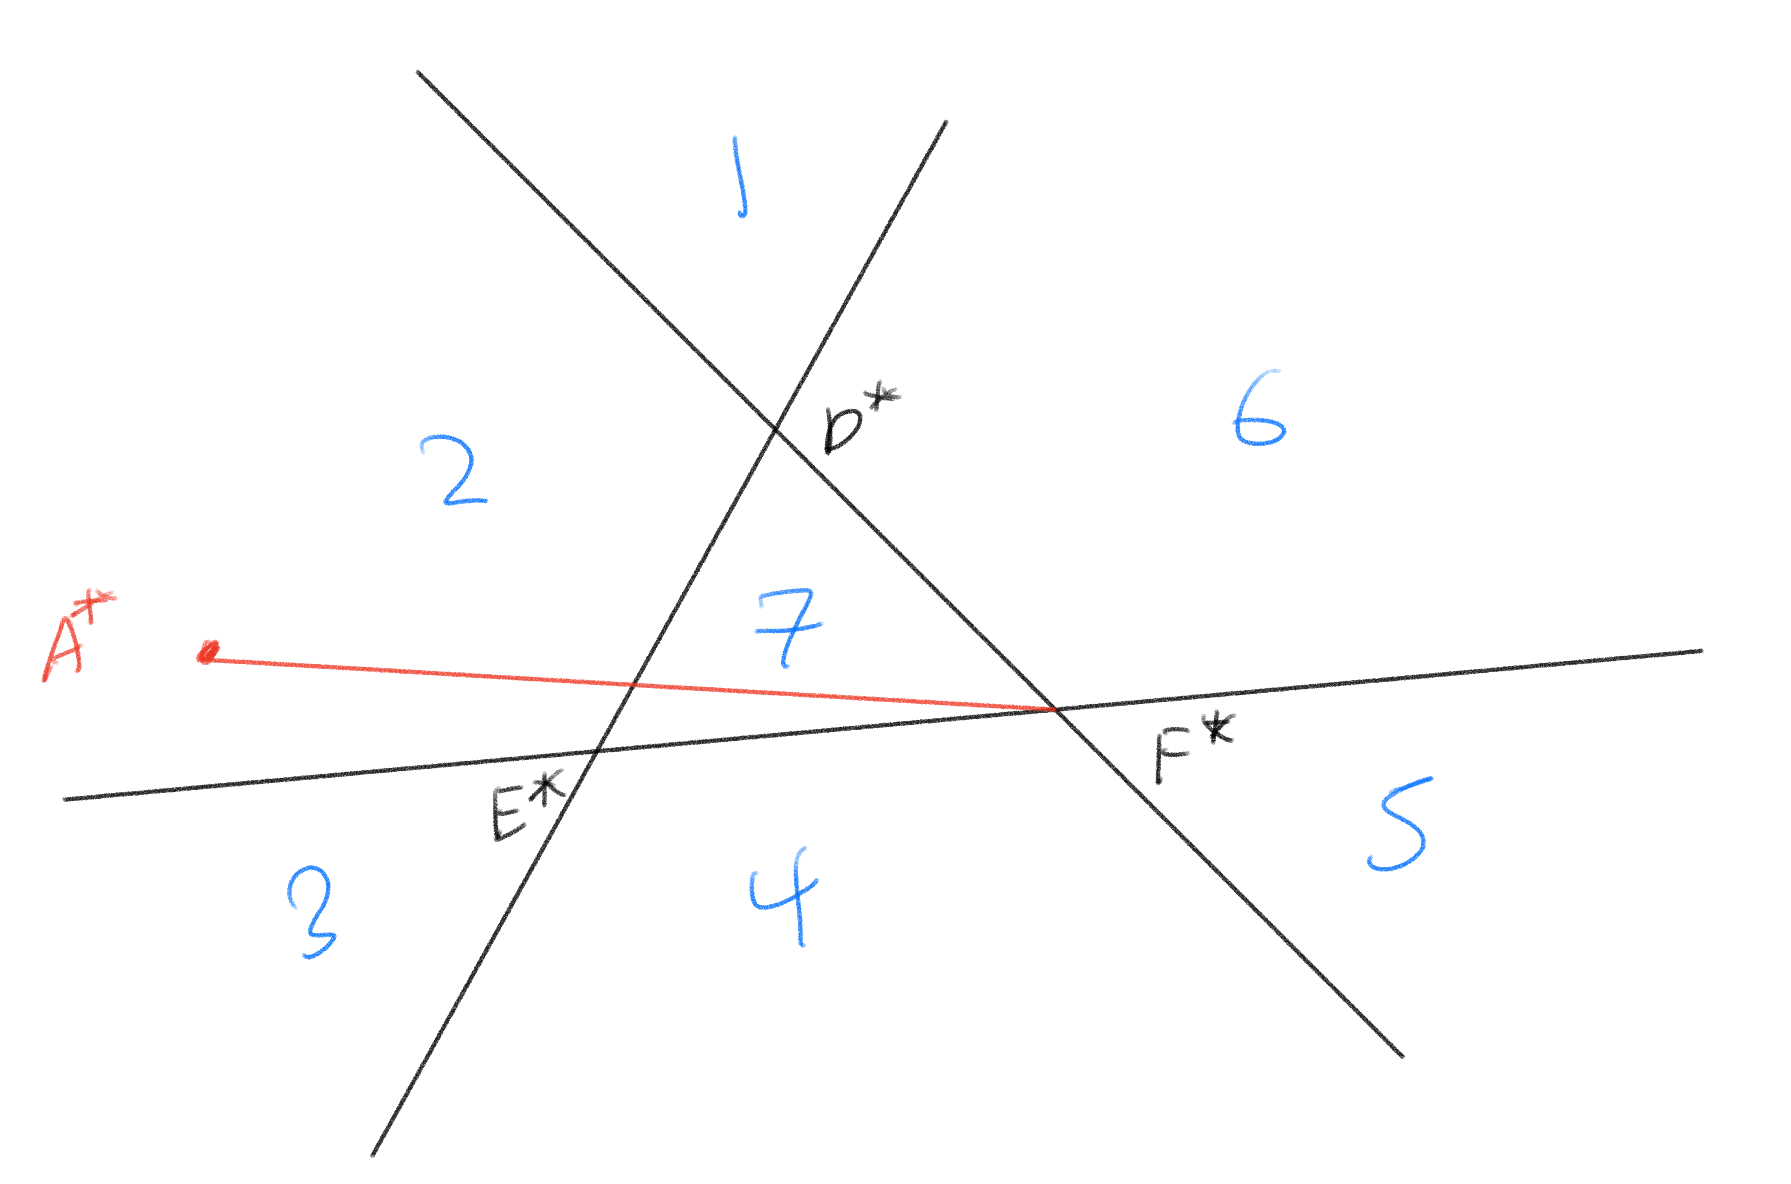
\includegraphics[width=8cm]{round3/p4diagram_3.jpeg}
\end{center}

We can now assume that points $A^*$, $B^*$, and $C^*$ will only occupy regions 1,3, or 5.

If $A^*$, $B^*$, and $C^*$ all reside on one of these regions, say region 1, then the set of points that can be in the interior of $\triangle A^*B^*C^*$ is a subset of region 1 (because region 1 is convex). But $E^*$ is not in region 1 (when it must be an interior point of $\triangle A^*B^*C^*$), which is a contradiction.

This means that at least two of the regions need to be occupied. Without loss of generality, assume that $A^*$ is in region 1 and $B^*$ is in region 3. Then, $A^*D^*E^*B^*$ is a convex quadrilateral. In particular, points $D^*$ and $B^*$ must be on opposite sides of the line $A^*E^*$ or on the line, and points $A^*$ and $E^*$ need to be on opposite sides of the line $B^*D^*$ or on the line. Therefore, this quadrilateral cannot be concave.

\begin{center}
    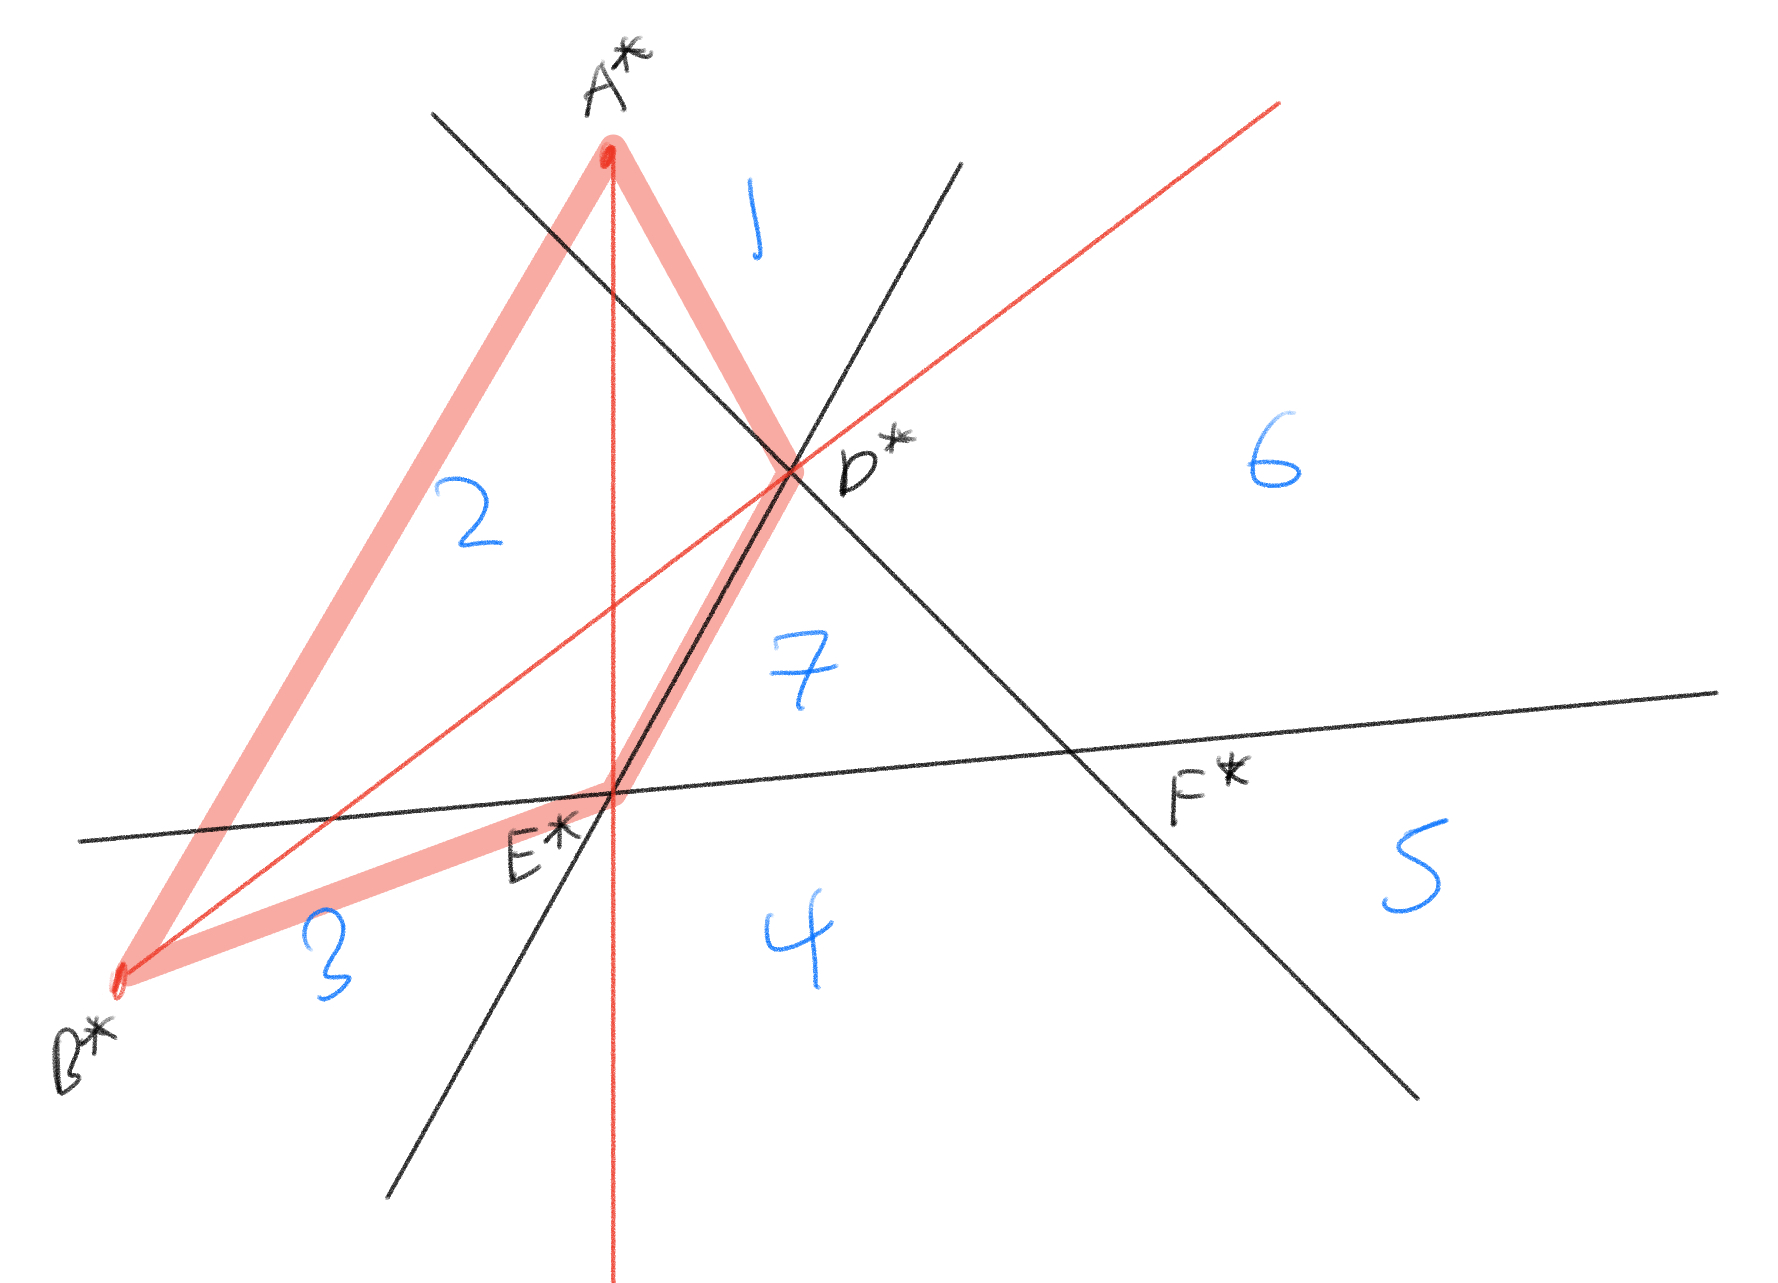
\includegraphics[width=8cm]{round3/p4diagram_2.jpeg}
\end{center}

Therefore, there will always exist a convex quadrilateral whose image under $f$ is a convex quadrilateral.
\hfill\qed
\end{solution}

%%%%%%%%%%%%%%%%%%%%%%%%%%%%%%%%%%%%%
%%%%%%%%%%                 %%%%%%%%%%
%%%%%%%%%%    Problem 5    %%%%%%%%%%
%%%%%%%%%%                 %%%%%%%%%%
%%%%%%%%%%%%%%%%%%%%%%%%%%%%%%%%%%%%%
\begin{solution}
The answer is the set of points that are on the ellipsoid with equation $x^2 + y^2 + 2z^2 = 1$ such that $z \neq 0$.

Let us consider a triangle $\triangle ABC$. For the perpendicularity conditions to hold, $P$ needs to lie on a sphere with radius $\frac{BC}{2}$ and centered at the midpoint of $\overline{BC}$. Let this sphere be denoted $\Gamma_A$, and define $\Gamma_B$ and $\Gamma_C$ likewise. Note that $\Gamma_A$ is the locus of all points $X$ such that $BX \perp CX$, and likewise for $\Gamma_B$ and $\Gamma_C$. We would like to find points where all three circles concur.

Because of this definition, $\Gamma_B$ and $\Gamma_C$ will pass through $A$ and the foot of the perpendicular line from $A$ to $BC$ (which we will temporarily denote $D$). Therefore, the locus of all points that are on both $\Gamma_B$ and $\Gamma_C$ will be a circle with diameter $AD$ and which is perpendicular to the xy plane. So, the projection of $P$ onto the xy plane, mapping from $(x,y,z) \rightarrow (x,y,0)$, must be on segment $AD$. We repeat the same reasoning for the other two cases. Therefore, the projection of $P$ is on the orthocenter of $\triangle ABC$ (denoted $H$), and it can only exist if $\triangle ABC$ is acute.

Now, we would like to calculate the length of $HP$. Let $M$ be the midpoint of $BC$. Since $M$ is the center of $\Gamma_A$ and $P$ is the concurrency point of all three circles, $MP = MB = MC$. Therefore, $HP^2 = MB^2 - MH^2$. To calculate this, we will use complex numbers. Let our unit circle be the complex unit circle and let $a,b,c$ denote the three points of $\triangle ABC$. Now, $M$ is defined as $\frac{b+c}{2}$ and $H$ is defined as $a+b+c$.

\newcommand{\ol}{\overline}

\begin{align*}
    MB^2 &= \paren{b - \frac{b+c}{2}}\paren{\ol{b} - \ol{\frac{b+c}{2}}}\\
         &= \paren{\frac{b-c}{2}}\paren{\frac{\ol{b}-\ol{c}}{2}}\\
         &=\frac{2-\ol{b}c-b\ol{c}}{4}\\
\end{align*}

\begin{align*}
    -MH^2 &= -\paren{a+b+c - \frac{b+c}{2}}\ol{\paren{a+b+c - \frac{b+c}{2}}}\\
          &= -\paren{a + \frac{b+c}{2}}\paren{\ol{a}+\frac{\ol{b}+\ol{c}}{2}}\\
          &= -1 + \frac{-a\ol{b}-a\ol{c}}{2} + \frac{-\ol{a}b-\ol{a}c}{2} + \frac{-2-b\ol{c}-\ol{b}c}{4}\\
\end{align*}

Summing these two expressions together, we get that
\begin{align*}
    HP^2 &= \frac{-2 - a\ol{b}-\ol{a}b -a\ol{c}-\ol{a}{c} - b\ol{c}-\ol{b}{c}}{2}\\
         &= \frac{1 - \paren{a+b+c}\paren{\ol{a}+\ol{b}+\ol{c}}}{2}\\
         &= \frac{1 - OH^2}{2}\\
\end{align*}

Which shows all possible values of the $z$-coordinate of $P$ (given a fixed $\triangle ABC$), as desired. Since our expression for $P$ is symmetric to $a$, $b$, and $c$, it follows that we can apply the same computations for $\Gamma_B$ and $\Gamma_C$ and get the same result for $HP^2$. Therefore, $P$ is the concurrency point of all three circles.

We have one edge case, where $\triangle ABC$ is a right triangle. Without loss of generality, let $\angle ABC = 90^\circ$. Then, the orthocenter coincides with $B$, and because of our computations before, $P$ should also coincide with $B$ as well (since it is on the z-axis). However, the angle $\angle BPC = \angle BBC$ is not well-defined in and of itself.

The problem now finishes with the following claim:

\begin{claim}
    All points on the open unit disk are an orthocenter of some non-obtuse triangle.
\end{claim}
\begin{proof}

\begin{figure}
\centering
    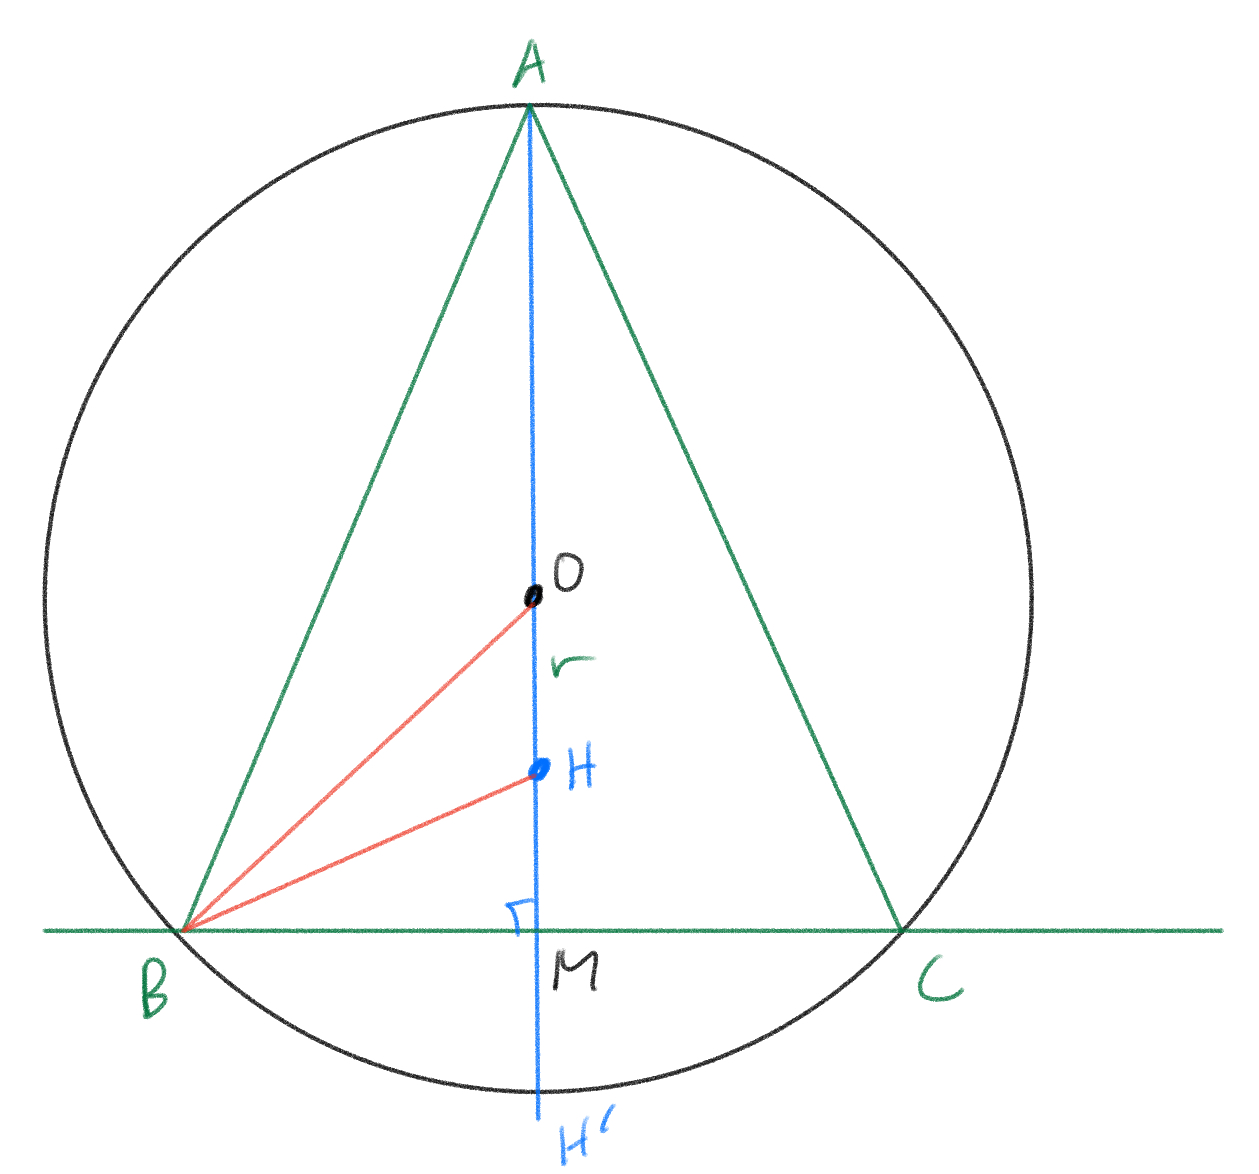
\includegraphics[width=8cm]{round3/p5construct.jpeg}
\end{figure}
    Let the distance from $O$ to $H$ be denoted $r$. Extend ray $OH$ (if $O=H$, any ray from $O$ will suffice) to meet the unit circle again at $H'$. Let $M$ be the midpoint of $HH'$. Let $A$ be the antipode of $H'$ and $B$ and $C$ the intersections of the perpendicular bisector of $HH'$ with the unit circle. Since $O$ is inside our triangle, it follows that $\triangle ABC$ is acute. By Power of Point, $H'M \cdot AM = HM \cdot AM = MB \cdot MC$. This implies that $\frac{MB}{HM} = \frac{AM}{MC}$, and so $\triangle AMC \sim \triangle BMH$. Since $HM \perp MC$, it follows that $BH \perp AC$. The same reasoning applies on the other side by symmetry, so $H$ is the orthocenter of $\triangle ABC$.
\end{proof}

\end{solution}

\end{document}